\documentclass[12pt]{article}
\usepackage{titling}
\usepackage{graphicx}
\usepackage{caption}
\usepackage{subcaption}

\newcommand{\subtitle}[1]{%
  \posttitle{%
    \par\end{center}
    \begin{center}\large#1\end{center}
    \vskip0.5em}%
}

				

\begin{document}

%

\title{Distance between two Causal Arcs of a Causal Belief System}			% used by \maketitle
\author{Johannes  Castner, }		% used by \maketitle
\date \today	
\maketitle
  \begin{abstract}
Diversity within organizations or political groups is often discussed in the recent literature for various reasons, such as diversity's theorized role in the success of an organization (Hong and Page 2004). This current work constructs an empirical measure of cognitive diversity, defined as the diversity of mental models, in order to facilitate confronting theories of diversity with evidence.  A person's mental model is represented as a directed labeled graph, where the nodes are discussed concepts and the directed edges between them are asserted causal relations (as in Axelrod 1976).  Using a newly developed computational linguistics tool (which is first used and presented as a part this work), these objects can be automatically extracted from very large texts, allowing for an accurate measurement of a quantity that might otherwise seem illusive: a group's cognitive diversity. 
  \end{abstract}

\subsection{A Distance Measure for a Single Arc in a Causal Belief System}

\begin{figure}
        \centering
      
             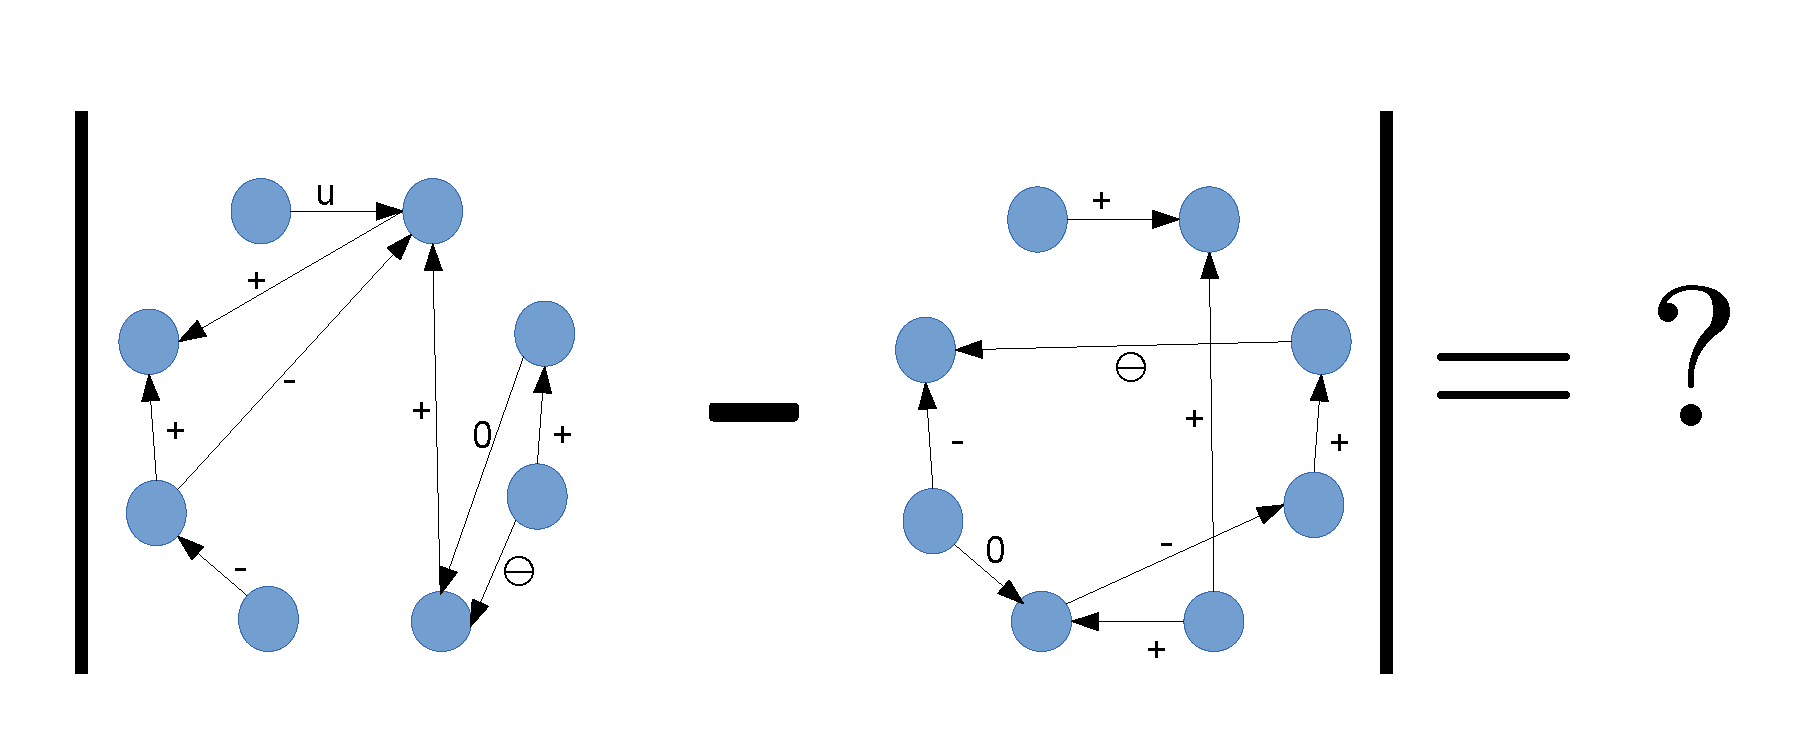
\includegraphics[width=\textwidth]{GraphDistance.pdf}
             \caption{How can we calculate a numerical difference between two belief systems, when belief systems are represented as signed digraphs?}
                
               \end{figure}%
   
In any political text it is natural to distinguish between seven causal relations that could exist between any two concepts:

\begin{itemize}
\item $+$: positive
\item $-$: negative
\item $\oplus$: non-negative
\item $\ominus$: non-positive
\item $0$: zero
\item $m$: non-zero (positive or negative)
\item $u$: universal (positive, zero, or negative)
\end{itemize} 

When a speaker does not assert a relationship at all, it can either be the case that she finds no relationship (a zero relationship) between the two concepts, or that she does not know the sign of such a relationship at all (the relationship is ambiguous to her). As will become clear momentarily, the difference between ambiguity and a zero relation can be quite important. Thus, if a person never speaks about the concepts in question, ambiguity should be assumed, whereas if the speaker refers to the concepts quite often, but never to a relation between them, then a $0$ relation should be assumed (she knows about the importance of the concepts but believes that no relation between them exists; otherwise, she would have stated such a relationship).  

I assume, as do many cognitive scientists (Tenenbaum, Griffiths, etc.) that each politician holds a belief system with which she understands her world and that this belief system is akin to a Bayesian Net, where the nodes of the directed graph are cause and effect concepts and the relations between these concepts are believed causal effects.  Each arc of this graph then, can be understood as a probabilistic causal effect from a cause to an effect variable, with a point estimate around which the causal belief is centred and some uncertainty surrounding this point estimate.  Other people, however, including researchers who wish to understand the speaker's beliefs, only observe statements about beliefs that are much coarser than the full Bayesian net (the seven types of relations that are discussed above).  In order to build a measure of the diversity of belief systems (a group level measure) I must then estimate the distance between any two belief systems (Weitzman 1992). The distance between two belief systems aggregates the distances between all individual beliefs regarding the same relationships using a generalization of the Hamming distance.  The distance between two people's believed relationships regarding the same two concepts is approximated as follows: \footnote{Aside from being theoretically plausible, this approach has the merit of allowing for easy robustness checks; for example, the seven relationships can easily and meaningfully be collapsed into fewer types of relations, such as '+', '0', '-' and 'u'.} 


The two dimensional belief space, with respect to a single causal relation, can be parsimoniously represented as the plane defined by two parameters, $\mu$ the causal effect estimate, or mean belief, and $\sigma$, the uncertainty parameter associated with this belief. Differences between two peoples' beliefs can then simply be interpreted as the Euclidean distance in this space.  While, for obvious reasons, an exact distance can not be calculated, by graphically inspecting the space, it becomes clear how the distances should be ordered on an ordinal scale and by changing the weighting scheme (making certain distances larger and others smaller) a simple robustness check can be devised, which also includes the possibility of meaningfully collapsing some of the categories of beliefs (a non-negative belief can be collapsed with a positive belief, for example). For example, the distance between a positive and a negative belief with respect to a pair of concepts can be calculated in theory as

$$d(+, -)=\sqrt{(\mu_{+}-\mu_{-})^2 + (\sigma_{+}-\sigma_{-})^2},$$      

but in practice we must put numbers on the parameters, $\mu_{+}, \mu_{-}, \sigma_{+}, \sigma_{-}, \mu_{0}, \sigma_{0}, \mu_{ambiguous}, \sigma_{ambiguous}$ etc. which then determine the distances. Assigning numbers to these parameters seems arbitrary, but as long as the ordinal distances between these regions make sense this arbitrariness is immaterial (as distances and diversity are only ordinal measures and I can use robustness checks to assure that the ordinal rankings are preserved). To begin with, I assign $\mu_{-}=\mu_{\ominus}=-2$ and $\sigma_{-}=0$, $\sigma_{\ominus}=1$ so that only the uncertainty between a non-positive and a negative statement differs, but the mean belief is the same. I then assign $\mu_{0}=0$, which is natural and $\sigma_{0}=1$. This gives $d(-, \ominus)=1$, $d(-, 0)=\sqrt{2+1}=\sqrt{3}$, $d(\ominus, 0)=\sqrt{2}.$ The positive spectrum of statements is symmetric and thus I will not enumerate all the cases; it suffices to say that the difference between a positive and a negative statement is as follows $d(-, +)=\sqrt{-2-2}=2.$ For the ambiguous statement, I let $\mu_{ambiguous}=0$ and $\sigma_{ambiguous}=2$, so that $d(0, ambiguous)=1$, $d(-, ambiguous)=\sqrt{2 + 2}=2$, etc. All of these parameters will of course be varied in the analysis, to see how much the exact numbers matter for the ordinal ranking of diversity measures for each of the two American political parties over time.      

\begin{figure}
        \centering
        \begin{subfigure}[b]{0.5\textwidth}
                \centering
                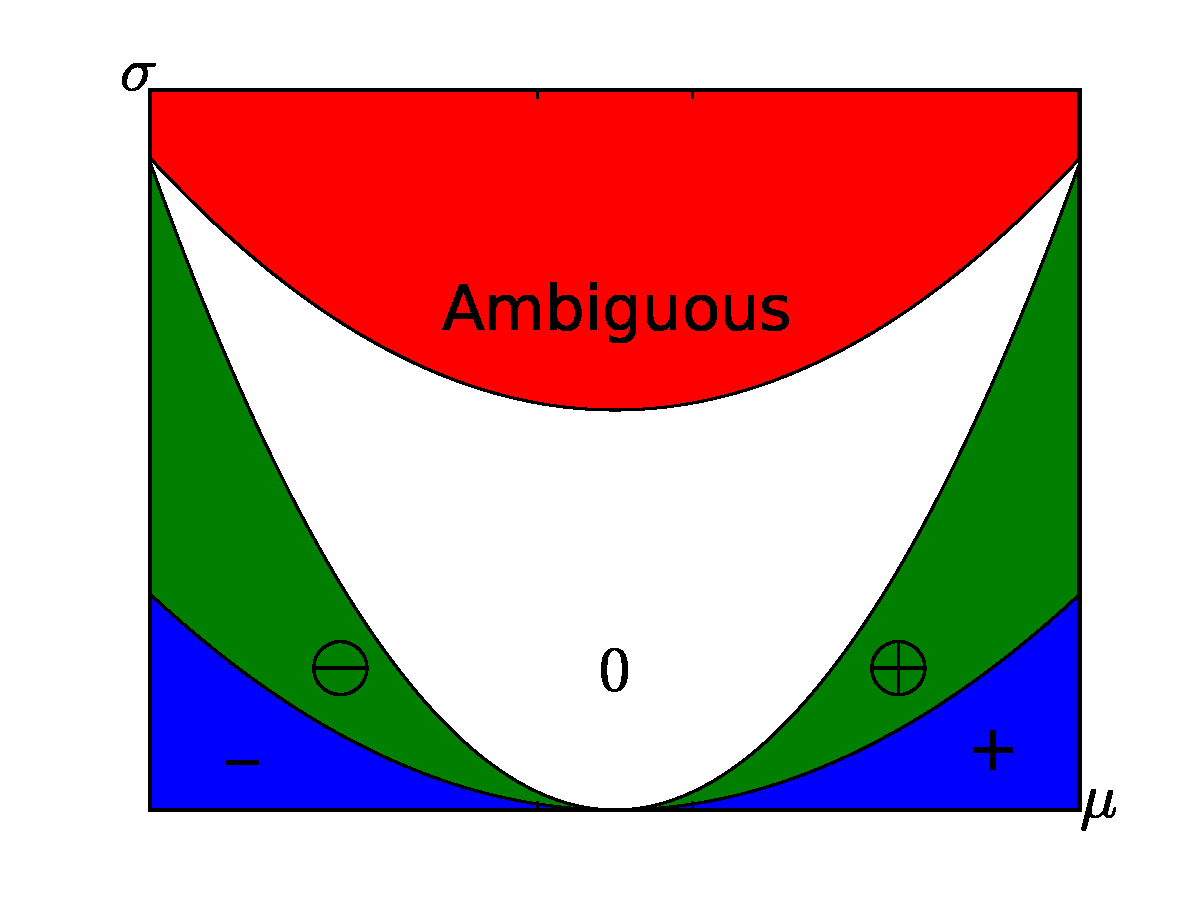
\includegraphics[width=\textwidth]{priors.pdf}
                \caption{the belief space}
                \label{fig:space}
        \end{subfigure}%
        ~ %add desired spacing between images, e. g. ~, \quad, \qquad etc.
          %(or a blank line to force the subfigure onto a new line)
        \begin{subfigure}[b]{0.5\textwidth}
                \centering
                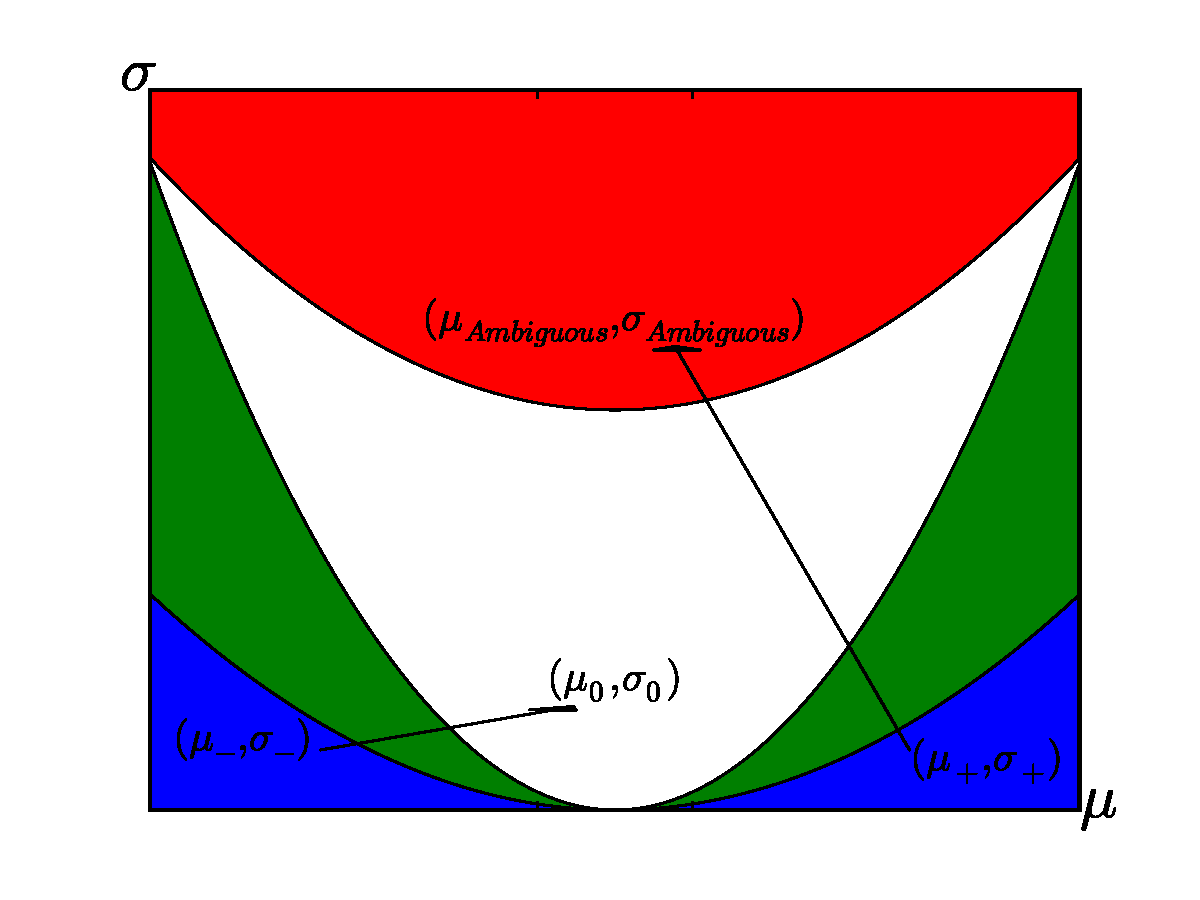
\includegraphics[width=\textwidth]{distances.pdf}
                \caption{distances between beliefs}
                \label{fig:dist}
        \end{subfigure}
        ~ %add desired spacing between images, e. g. ~, \quad, \qquad etc.
          %(or a blank line to force the subfigure onto a new line)
      \caption{The space of beliefs and distances between speakers' beliefs. The blue regions are those where a speaker believes in a (negative or positive) causal elation, in the green region, speakers weakly believe in relations. If the parameters fall in the white region, a speaker believes that there is likely no relation, whereas the red region defines the space of total ambiguity. For the purpose of taking distances, the regions are collapsed onto single points in the $(\mu, \sigma)$ space, which could be thought of as averages, but they can be streched for the purposes of robustness checks.}\label{fig:belief_space}  
\end{figure}

          

\end{document}             % End of document.
